\documentclass{article}
\usepackage[utf8]{inputenc}
\usepackage{amsthm}
\usepackage{amsmath, mathtools, amsfonts,amssymb}
\usepackage{graphicx}
\usepackage{verbatim}
\usepackage{fancyhdr}

\usepackage{subfigure}
% Code
\usepackage{listings} 
\usepackage{algorithm}
\usepackage[noend]{algpseudocode}
% Margins
\usepackage{geometry}
%\geometry{margin=1in} %% 
% Graphics
\usepackage{tikz}
\usetikzlibrary{matrix} % matrices
\usepackage{tikz-qtree} % Simple trees
% Theorems/etc.
\newtheorem{pic}{Figure}
\numberwithin{pic}{section}
\newtheorem{lem}{Lemma}
\numberwithin{lem}{section}
\newtheorem{thm}{Theorem}
\numberwithin{thm}{section}
\newtheorem{cor}{Corollary}
\numberwithin{cor}{section}
\theoremstyle{definition}
\newtheorem{ex}{Example}
\numberwithin{ex}{section}
\newtheorem{defn}{Definition}
\numberwithin{defn}{section}
\theoremstyle{definition}
\newtheorem{prob}{Problem}
\theoremstyle{remark}
\newtheorem*{con}{Conjecture}
\newtheorem{rem}{Remark}
\newtheorem*{cex}{Counterexample}
\newtheorem*{ts}{T.S.}

%%% COMMANDS %%%
% Sets
\newcommand{\set}[1]{\ensuremath{\left\{ #1\right\}}} % write sets
\newcommand{\e}{\ensuremath{\epsilon}} % Epsilon
\newcommand{\R}{\ensuremath{\mathbb{R}}} % Real Numbers
\newcommand{\C}{\ensuremath{\mathbb{C}}} % Complex Numbers
\newcommand{\N}{\ensuremath{\mathbb{N}}} % Natural numbers
\newcommand{\Q}{\ensuremath{\mathbb{Q}}} % Rationals
\newcommand{\I}{\ensuremath{\mathbb{I}}} % Irrational Numbers
\newcommand{\Z}{\ensuremath{\mathbb{Z}}} % Integers
% Easier Delimiters?
\newcommand{\lr}[2]{\ensuremath{\left#1 #2 \right #1}}
% Absolute Value
\newcommand{\abs}[1]{\ensuremath{\left| #1 \right|}}
% Landau Notation
\newcommand{\Oh}{\ensuremath{\mathcal{O}}} %%% IN MATH MODE
\newcommand{\oh}{\ensuremath{\mathcal{o}}} %%% IN MATH MODE
% Display style fractions
\newcommand{\Frac}[2]{\displaystyle \frac{#1}{#2}}
% Display style limits
\newcommand{\Lim}[2]{\displaystyle \lim_{#1}{#2}}

%% Norms %%
\newcommand{\norm}[1]{\ensuremath{\left | \left | #1 \right | \right |}}
%%% Preference Stuff %%%
\setcounter{section}{-1}
\renewcommand\qedsymbol{{$\blacksquare$}}
% Enumerate
\renewcommand{\labelenumi}{(\alph{enumi})}
\renewcommand{\labelenumii}{\roman{enumii}}
% change proof environment
\renewcommand*{\proofname}{Pf}
% Line Spacing
\renewcommand{\baselinestretch}{1.5}
% Indentation
\newlength\tindent
\setlength{\tindent}{\parindent}
\setlength{\parindent}{0pt}
\renewcommand{\indent}{\hspace*{\tindent}}
% Set title
\title{Computational Math Project\\
  {\large Illinois Institute of Technology}
}
\author{
  Miles Bakenhus 
  \and
  Ahmed Lodhika 
  \and
  Gunjan Sharma 
  \and
  Quinn Stratton 
  \and
  Jan-Eric Sulzbach 
}
\date{\today}
\begin{document}
\fancyhead[l]{}
\fancyhead[c]{}
\fancyhead[r]{}
% \pagestyle{fancy}
\maketitle
\newpage
\tableofcontents
\section{Introduction}

\section{Origin of the problem and its applications}
In this part of the project we explain the motivation behind our ideas and consider the applications of the results.\\
First, we consider the standard elliptic equation in two dimensions
\begin{align*}
-\Delta u &= f ~\text{ in } \Omega\\
u&=0 ~\text{ on } \partial\Omega.
\end{align*}
Then the discretised equation on a grid is
\begin{align*}
-\Delta_h u_{ij} &= f_{ij} ~\forall\,(x_i,y_i)\in \Omega_h,~f_{ij}=f(x_i,y_j)\\
u_{ij}&=0 ~\forall\,(x_i,y_i)\in \partial\Omega_h,
\intertext{where we use the second order central differencing to represent the Laplace operator}
-\Delta_h u_{ij}= \Frac 1{h^2}\begin{pmatrix}
0 & -1 & 0 \\ 
-1 & 4 & -1 \\ 
0 & -1 & 0
\end{pmatrix}u_{ij}&= \Frac 1{h^2} \big(-u_{ij+1}-u_{i-1j}+4 u_{ij}-u_{i+1j}-u_{ij_1}\big)
\end{align*}
If we assume that the domain $\Omega$ is a square and ordering the grid points from left to right and bottom to top yields the following matrix of the system $A\in \R^{(h-1)^{-2}\times (h-1)^{-2}}$:
\[A=h^2\begin{pmatrix}
4 & -1 & 0 & \dots & 0 & -1 &  &  \\ 
-1 & 4 & -1 &  &  &  & \ddots &  \\ 
0 & -1 & 4 & \ddots &  &  &  & -1 \\ 
\vdots  &  & \ddots & \ddots &  &  &  & 0\\ 
0 &  &  &  &  &  &  & \vdots \\ 
-1 &  &  &  &  & \ddots & \ddots & 0 \\ 
 & \ddots &  &  &  & \ddots & 4 & -1 \\ 
 &  & -1 & 0 & \dots & 0 & -1 & 4
\end{pmatrix} \]
And the problem we need to solve is the linear system $Au=f$.\\
Therefore it is important to understand how the structure of $A$ affects the structure of the $QR$ decomposition.
Note that in this case the highest and lowest off-diagonal has a distance of order   $h$ from the diagonal.\\

Another example where these banded matrices show up is in the following:
Consider the parabolic equation in two dimensions
\[\frac{\partial u}{\partial t}=\sigma \Delta u,~ 0\leq x\leq X,\, 0\leq y\leq Y\, 0\leq t\leq T\]
with Dirichlet boundary condition and a given initial data $u(x,y,0)=U^0(x,y)$.\\
For the numerical implementation we consider the implicit Crank-Nicolson scheme
\begin{align*}
&-\frac{\mu_x}{2}\big(U_{j-1,l}^{n+1}+ U_{j+1,l}^{n+1}\big) -\frac{\mu_y}{2}\big(U_{j,l-1}^{n+1}+U_{j,l+1}^{n+1}\big)+\big(1+\mu_x+\mu_y\big)U_{j,l}^{n+1}\\
=&\frac{\mu_x}{2}\big(U_{j-1,l}^{n}+ U_{j+1,l}^{n}\big) +\frac{\mu_y}{2}\big(U_{j,l-1}^{n}+U_{j,l+1}^{n}\big)+\big(1-\mu_x-\mu_y\big)U_{j,l}^{n},
\end{align*}
for $0\leq j\leq J_x$, $0\leq l\leq J_y$ and $n>0$.
Again we can rewrite this as a linear system $AU^{n+1}=U^n$, where 
\[A=\begin{pmatrix}
1+\mu_x+\mu_y & -\frac{\mu_x}{2} & 0 & \dots & 0 & -\frac{\mu_y}{2} &  &  \\ 
-\frac{\mu_x}{2} & 1+\mu_x+\mu_y & -\frac{\mu_x}{2} &  &  &  & \ddots &  \\ 
0 & -\frac{\mu_x}{2} & 1+\mu_x+\mu_y & \ddots &  &  &  & -\frac{\mu_y}{2} \\ 
\vdots  &  & \ddots & \ddots &  &  &  & 0\\ 
0 &  &  &  &  &  &  & \vdots \\ 
-\frac{\mu_y}{2} &  &  &  &  & \ddots & \ddots & 0 \\ 
 & \ddots &  &  &  & \ddots & 1+\mu_x+\mu_y & -\frac{\mu_x}{2} \\ 
 &  & -\frac{\mu_y}{2} & 0 & \dots & 0 & -\frac{\mu_x}{2} & 1+\mu_x+\mu_y
\end{pmatrix} \]
and $A\in\R^{(J_x-1)(J_y-1)\times (J_x-1)(J_y-1)}$ where the highest and lowest off-diagonal band have the distance $J_x-1$ from the diagonal.
\begin{rem}
In the case of three dimension, we would obtain one more non-zero sub/super-diagonal, now with a distance of $\mathcal{O}(J_x*J_y)$ from the diagonal.
\end{rem}

\section{Matrix Properties}
\subsection{Tridiagonal Matrices}
\begin{thm}
If $A$ is a tridiagonal matrix. Then R in the the product $A=QR$ is a upper triangular matrix with non zero entries only in the diagonal and the two super diagonals.
\end{thm}
\[A=\begin{pmatrix}
a_{11} & a_{12} &  &   \\ 
a_{21} & a_{22} & a_{23} &    \\ 
 & \ddots & \ddots & \ddots   \\ 
   &  & a_{m m-1} & a_{mm}
\end{pmatrix}~,~R=\begin{pmatrix}
r_{11} & r_{12} & r_{13} &  \\ 
 & \ddots & \ddots & \ddots \\ 
 &  & \ddots & \ddots \\ 
 &  &  & r_{mm}
\end{pmatrix}  \]
\begin{proof}
To prove the statement we will use the classical Gram-Schmidt method for the QR decomposition.\\
Step 1: we want to show that $q_j$ has the form $q_j=\begin{pmatrix}
* \\ 
\vdots \\ 
* \\ 
0 \\ 
\vdots
\end{pmatrix} \leftarrow j+1\text{-th entry}$.\\
We prove this by induction:
\begin{description}
\item[Base step] $j=1$ the if we assume that $\|a_1\|=1$ then $q_1=a_1$ thus
\[q_1= \begin{pmatrix}
a_{11} \\ 
a_{21} \\ 
0 \\  
\vdots
\end{pmatrix}\]
\item[Induction step] Assume that the statement holds for $j-1$. Then
\[v_j=a_j-\sum_{k=1}^{j-1} (q_k^* a_j)q_k~\text{ and } q_j= v_j/\|v\|_j\]
and by using the form of $q_{j-1}$ we obtain
\[q_j= \begin{pmatrix}
0\\ 
\vdots \\ 
a_{j-1, j} \\ 
a_{jj} \\ 
a_{j+1,j} \\
0\\
\vdots
\end{pmatrix}-\sum_{k=1}^{j-1} \begin{pmatrix}
*\\ 
\vdots \\ 
\vdots \\ 
* \\ 
0 \\
\vdots\\
\vdots
\end{pmatrix}\leftarrow k+1\text{-th entry}= \begin{pmatrix}
*\\ 
\vdots \\ 
\vdots \\ 
* \\ 
0 \\
\vdots\\
\vdots
\end{pmatrix}\leftarrow j+1\text{-th entry} \]
\end{description}
Step 2: Compute $r_{ij}$ in the CGS method\\
For $j=1$ to $n$ and for $i=1$ to $j-1$: $r_{ij}= q_i^*a_j$.
Then by step 1 we obtain that $r_{ij}=0$ if $i\leq j-3$ since then by the form of the vectors $q_{j-3}$ and $a_j$
\[0=\begin{pmatrix}
* \\ 
\vdots  \\ 
* \\ 
0 \\ 
0 \\
0\\
0 \\
\vdots \\ 
0
\end{pmatrix}^*\begin{pmatrix}
0 \\ 
\vdots  \\ 
0 \\ 
* \\ 
* \\ 
*\\
0\\
\vdots\\
0
\end{pmatrix} \leftarrow j\text{-th enttry} \]
The above argument holds for all $i\leq j-3$. 
\end{proof}
\subsection{General Banded Matrices}

\begin{proof}
  
Let $A = QR$ for $A,Q \in \C^{m \times m}$, $R \in \C^{m \times m}$, unitary $Q$, and upper triangular $R$. If $A$ has bandwidth $2p +1$ then for $i - j > p$, 
	$$ 0 = a_{ij} = \sum_{k = 1}^{m} q_{ik}r_{kj}$$
Since $R$ is upper triangular, $r_{kj} = 0$ for $k > j$. Then when $i > j + p$,
	$$ 0 = a_{ij} = \sum_{k = 1}^{j} q_{ik}r_{kj}$$
so $q_{ij} = 0$ . Hence 
	\begin{equation} \label{eq:1}
		q_{j} = \begin{pmatrix} 
			q_{1,j} \\
			q_{2,j} \\
			\vdots \\
			q_{j+p,j} \\
			0 \\
			\vdots \\
			0 \\
		\end{pmatrix}
	\end{equation}

From (\ref{eq:1}) when $i+p < j - p -1$ (i.e., $j - i > 2p + 1$):
	$$
		r_{ij} = q_i^* a_j =\begin{pmatrix}
			q_{1,i} & q_{2,i} &	\dots & q_{i+p,i} & 0 & \dots &	0 
		\end{pmatrix}\begin{pmatrix} 
		0 \\
		\vdots \\
		0 \\
		a_{j-p-1,j} \\
		\vdots \\
		a_{j+p+1,j} \\
		0 \\
		\vdots \\
		0 \\
		\end{pmatrix} = 0
	$$
Hence $R$ is upper triangular with its only nonzero entries in the diagonal and $2p$ super diagonals.
\end{proof}
\begin{figure}[H] 
    \subfigure[A]{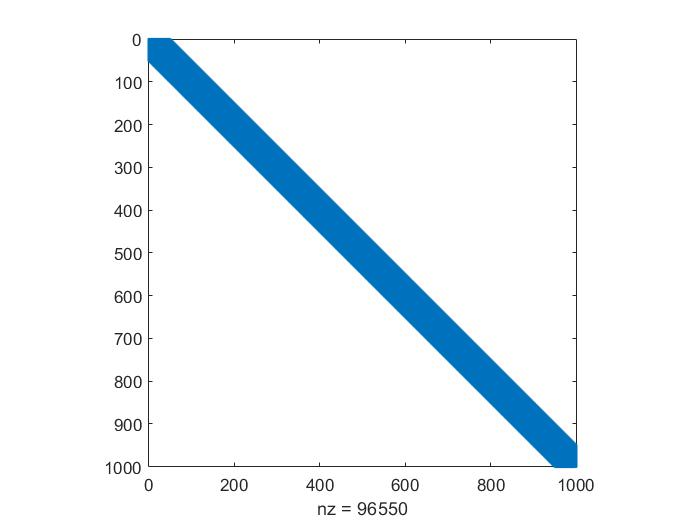
\includegraphics[width=0.49\textwidth]{example 8.jpg}} 
    \subfigure[R]{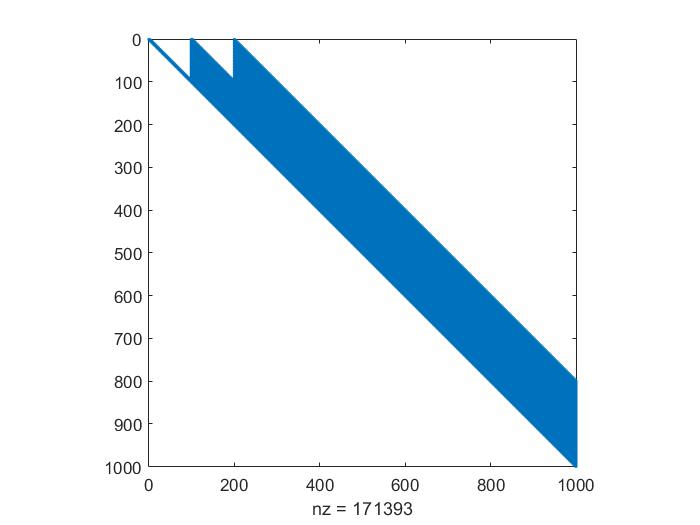
\includegraphics[width=0.49\textwidth]{example 9.jpg}}  

    \caption{bandwith 101, i.e $p=50$}
\end{figure} 
\begin{rem}
This results also holds for the matrices considered in the first part, i.e. the matrices derived from finite difference methods.
\end{rem}
\begin{figure}[H] 
    \subfigure[A]{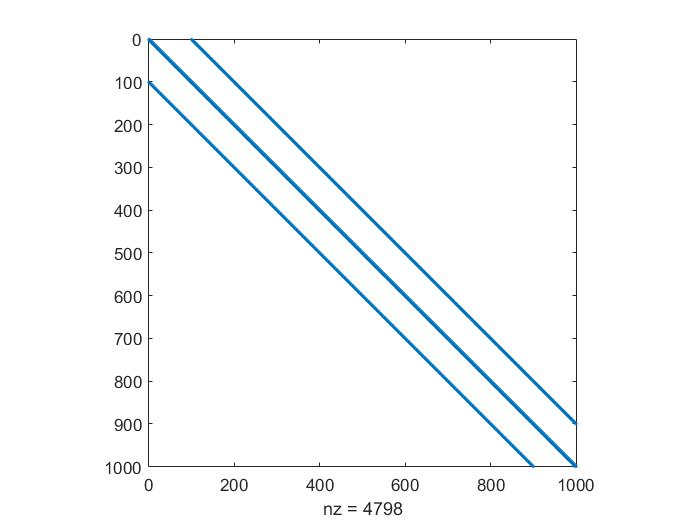
\includegraphics[width=0.49\textwidth]{example 6.jpg}} 
    \subfigure[R]{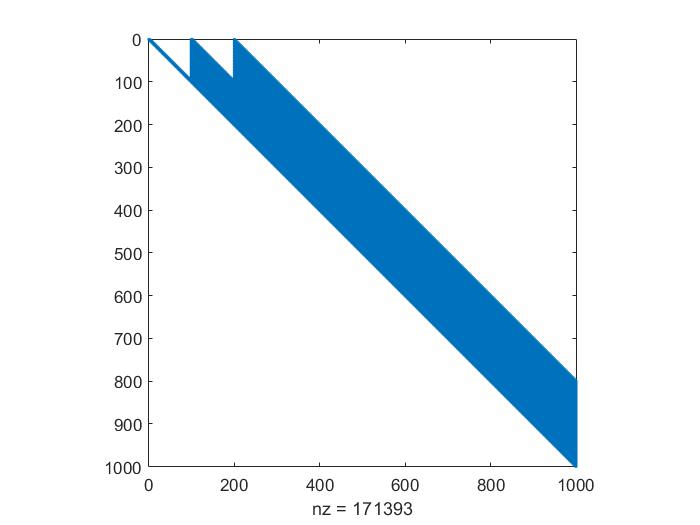
\includegraphics[width=0.49\textwidth]{example 7.jpg}}  

    \caption{A has the special form as in Section 1}
\end{figure} 
\subsection{Sparse Diagonal Matrices}
Now we want to generalize the above ideas to the case where A still has only three non-zero bands.
But now, the lower band has the distance $k-1$ from the diagonal and the upper band has the distance $l-1$ from the diagonal.\\
Consider the following example for A: 
\begin{figure}[	H]
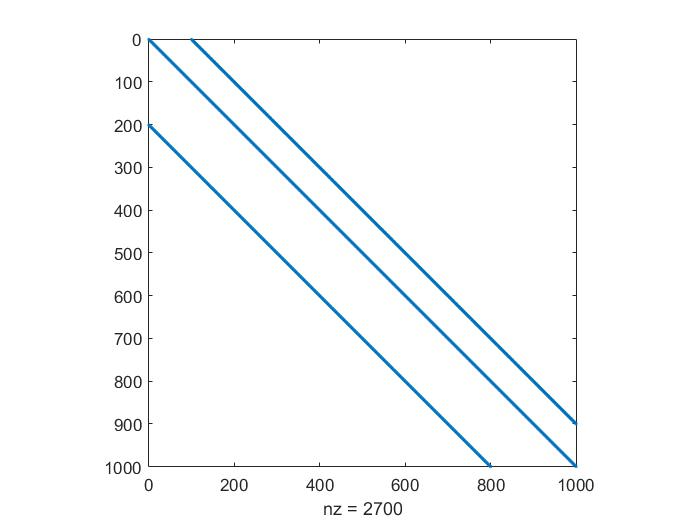
\includegraphics[scale=0.3]{example1.jpg}
\caption{$k=200$ and $l=100$}
\end{figure}

\begin{thm}[General case]
The upper triangular matrix $R$ in the $QR$ decomposition of $A$ has a $k+l$-band structure.
\end{thm}
\begin{proof}
From the classical Gram Schmidt method we immediately see, that in the worst case, the first $j+k$ entries are non zero.
Therefore, the inner product in the computation of the entries $r_{ij}$ is only zero if $i<j-l-k+2$. 
\end{proof}
Example of a matrix close to the worst case, where the number of non-zero entries (nz) increases by order 50:
\begin{figure}[H] 
    \subfigure[A]{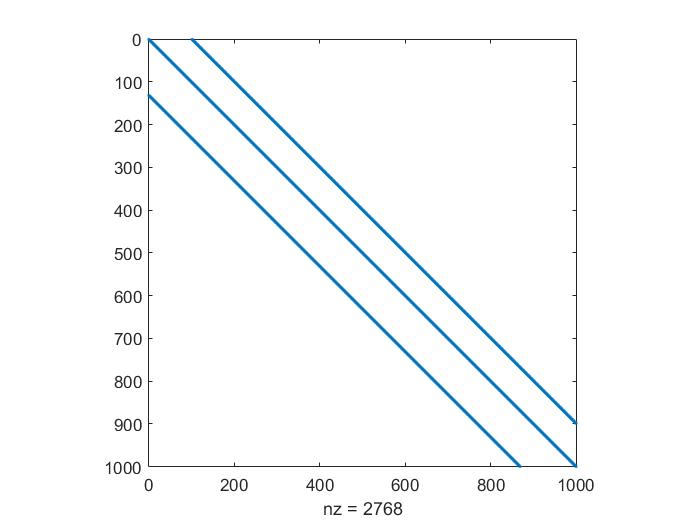
\includegraphics[width=0.49\textwidth]{example2.jpg}} 
    \subfigure[R]{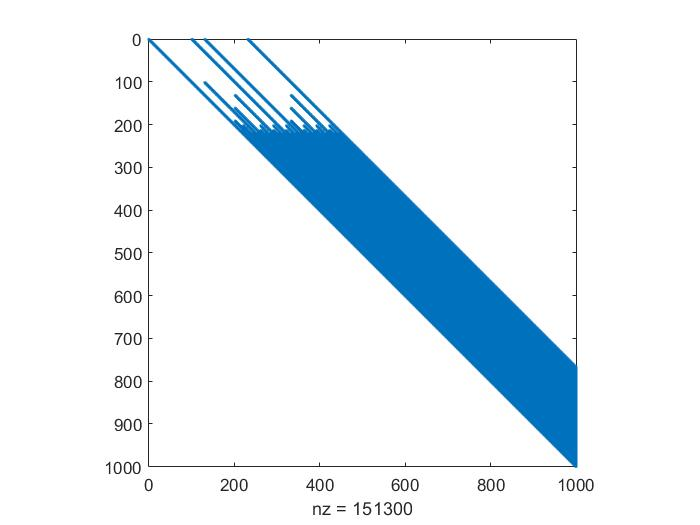
\includegraphics[width=0.49\textwidth]{example3.jpg}}  

    \caption{$k=131$ and $l=101$}
\end{figure} 
A special case occurs when $k=l$. Then again $R$ has only three non-zero band, i.e the diagonal, the band on the upper diagonal that has a distance $k$ to the diagonal and the upper diagonal that has a distance $2k$ to the diagonal.\\
Again we have an example for this case:
\begin{figure}[H] 
    \subfigure[A]{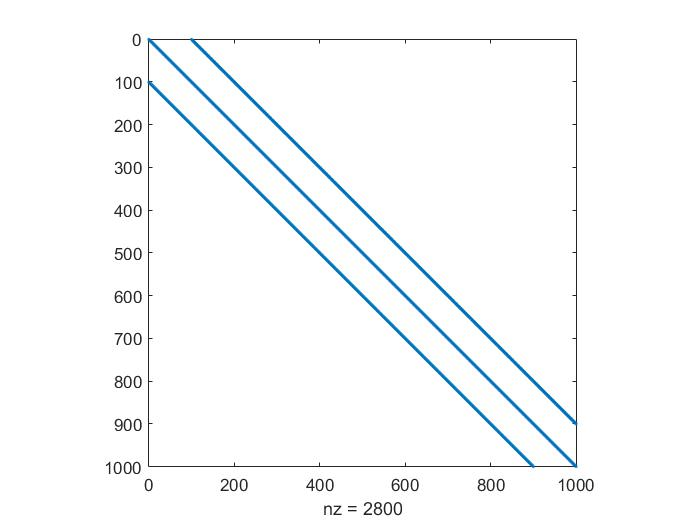
\includegraphics[width=0.49\textwidth]{example4.jpg}} 
    \subfigure[R]{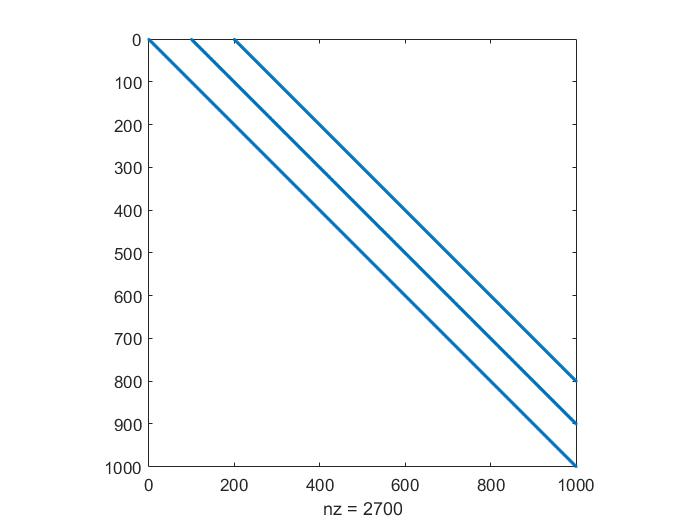
\includegraphics[width=0.49\textwidth]{example5.jpg}}  

    \caption{$k=l=100$ }
\end{figure} 
\begin{cor}
Let the square matrix $A$ have the form as mentioned in the example. 
Then $R$ of the $QR$ decomposition has the form $r_{ij}\neq 0$ only for the cases $i=j$, $i+k+1$ and $i+2k+2$.
\end{cor}
\begin{proof}
From the ideas of the theorems before, the column vector $q_i$ of $Q$ in the $QR$ decomposition has the form $q_i^*=(\underbrace{0\dots0}_{i\mod k}\,*\,\underbrace{0\dots0}_{k }\,*|\dots|*\,\underbrace{0\dots0}_{k}\,\underbrace{*}_{i-th}\,0\dots0\,*\,0,\dots)$.
Therefore $r_{ij}= q_i^* a_j=0$ for $i\neq j$ or $i+k+1\neq j$ or $i+2k+2\neq j$.
\end{proof}
\section{Algorithms and Results}
Based on the properties proved in the last section, it is fairly straightforward
to modify existing algorithms for finding a QR-factorization of a matrix to
exploit sparsity patterns.
\subsection{General Banded Matrices}
Suppose $A\in C^{m\times n}$ with bandwidth $p$. Consider some QR-factorization
of $A$, $A = QR$. Then by \textbf{THEOREM}, we
know that if $j > i + 2p$, $r_{ij} = 0$. We can alter the well-known
\textit{Modified Gram-Schmidt} algorithm to take advantage of the above fact in
the following way.
\begin{algorithm}[H]
  \caption{MGS for Banded Matrices}
  \begin{algorithmic}[1]
  	\For{$i = 1$\textbf{ to }$n$}
   	\State$v_i\gets a_i$
    \EndFor
    \For{$i = 1$\textbf{ to }$n$}
    \State$r_{ii}\gets \norm{\mathbf{v_i}}_2$
    \State$q_i\gets \mathbf{v_i} / r_{ii}$
    \For{$j = i + 1$\textbf{ to }$\text{min}\set{i + 2p, n}$}
    \State$r_{ij}\gets \mathbf{q_i}^*\mathbf{a_j}$
    \State$\mathbf{v_j}\gets\mathbf{v_j} - r_{ij}\mathbf{q_i}$
    \EndFor
    \EndFor
  \end{algorithmic}
  [Note that this is based on the \textit{Modified
    Gram-Schmidt} algorithm as described in \cite{nla}] 
\end{algorithm}
Below are some results for the performance of \textbf{MGS for Banded Matrices}
and the performance of the standard MGS algorithm applied to the same random
banded matrices.
\begin{center}
 Performance of \textit{Modified Gram-Schmidt} \textbf{NOT COMPLETE!}
\begin{tabular}{p{2cm}|p{2cm}p{2cm}p{2cm}p{2cm}p{2cm}p{2cm}p{2cm}}
    $\C^{10\times 10}$ & 0.0024461 &   0.0023396 &   0.0023416 &   0.0023403  &  0.0023373  &  0.0023707\\
    $\C^{500\times 500}$& 5.1399053  &  5.0569402   & 5.0526341  &  5.0476353 &   5.0430921  &  5.3553525\\
   $\C^{750\times 750}$& 12.0286885  & 12.1555834  & 12.3704160  & 12.0967193 &  12.5868144  & 12.2757503\\
  $\C^{1000\times 1000}$& 21.6673735  & 21.1107465  & 21.1824376  & 21.3300323  & 21.0178360  & 22.8876292 
\end{tabular}
\end{center}
\begin{center}
  \begin{tabular}{p{1cm}|p{2cm}p{2cm}p{2cm}p{2cm}p{2cm}p{2cm}p{2cm}}
    & & & & & &
  \end{tabular}
\end{center}
\subsection{Special Cases}
In the special case of the symmetric tridiagonal matrix $A$, where the super and sub diagonal have a distance $k$ from the diagonal, we can improve the \textbf{Algorithm 1} even further using \textbf{Theorem} and \textbf{Corollary}.
\begin{algorithm}[H]
  \caption{MGS for special tridiagonal Matrices }
  \begin{algorithmic}[1]
    \For{$i = 1$\textbf{ to }$n$}
   	\State$v_i\gets a_i$
    \EndFor
    \For{$i = 1$\textbf{ to }$n$}
    \State$r_{ii}\gets \norm{\mathbf{v_i}}_2$
    \State$q_i\gets \mathbf{v_i} / r_{ii}$ 
    \If{$i+2k+2\leq n$}
    	\State$r_{i,i+2k+2}\gets \mathbf{q_i}^*\mathbf{a_{i+2k+2}}$
    	\State$\mathbf{v_{i+2k+2}}\gets\mathbf{v_{i+2k+2}} - r_{i,i+2k+2}\mathbf{q_i}$
    	\State$r_{i,i+k+}\gets \mathbf{q_i}^*\mathbf{a_{i+k+1}}$
    	\State$\mathbf{v_{i+k+1}}\gets\mathbf{v_{i+k+1}} - r_{i,i+k+1}\mathbf{q_i}$
    	\ElsIf{$i+k+1\leq n$}
    	\State$r_{i,i+k+}\gets \mathbf{q_i}^*\mathbf{a_{i+k+1}}$
    	\State$\mathbf{v_{i+k+1}}\gets\mathbf{v_{i+k+1}} - r_{i,i+k+1}\mathbf{q_i}$
       	\EndIf
    \EndFor
  \end{algorithmic}
\end{algorithm}
\subsection{Flop count}
Here, we are going to give the theoretical flop count of the two algorithms and compare it with the MGS algorithm in \cite{nla}.\\
Recall that the MGS requires $\sim 2n^3$ operations, where the most amount of work is due to an inner \textit{for}-loop.
In both of the above algorithms we can eliminate/ heavily reduce the the size of the inner \textit{for}-loop.
Therefore the first algorithm has a flop count of $\sim 8*2pn^2$ and the second one for the special case tridiagonal matrices we have $\sim 8n^2$ flops.
\section{Further Study}

	\addcontentsline{toc}{section}{References}
	\bibliographystyle{unsrt}
	\bibliography{comp-math}
\end{document}
